\documentclass[12pt]{article}

\usepackage[english]{babel}
\usepackage[utf8]{inputenc}
\usepackage{sansmathfonts}
\usepackage[T1]{fontenc}
\renewcommand*\familydefault{\sfdefault} %% Only if the base font of the document is to be sans serif
\usepackage{multicol,lipsum}
\usepackage{amsmath,cancel}
\usepackage{amssymb,amsthm,dsfont,mathrsfs}
\usepackage[colorinlistoftodos]{todonotes}
\usepackage{geometry}
\geometry{
a4paper,
total={170mm,257mm},
left=20mm,
top=15mm,
bottom=22mm,
}
\usepackage{natbib}
\usepackage{soul}
\usepackage{setspace}
\usepackage{hyperref}
\usepackage{xcolor}
\usepackage{graphicx}
\usepackage{tikz}
\usepackage{siunitx}
\graphicspath{ {imagens/} }
\usepackage{fancyhdr}
\pagestyle{fancy}
\renewcommand{\headrulewidth}{0pt}

\color{darkgray}
\newcommand{\T}[1]{\vspace{0.4cm}\textbf{\large#1}}
\newcommand{\TW}[1]{\textbf{\large#1}}

\newcommand{\TM}[1]{\vspace{0.2cm} \textbf{#1}}

\newcommand{\M}[1]{
\vspace{-0.6cm}
\begin{flalign*}
#1&
\end{flalign*}
\vspace{-0.6cm}
}


\definecolor{bluebell}{rgb}{0.25, 0.35, 0.89} 
\definecolor{laranja}{rgb}{0.87, 0.48, 0.25} 
\definecolor{verde}{rgb}{0, 0.54, 0.44} 
\definecolor{babypink}{rgb}{1, 0.42, 0.52} 
\definecolor{rosa}{rgb}{1, 0.72, 0.77} 
\definecolor{cinza}{rgb}{0.3, 0.3, 0.3}  
\definecolor{iris}{rgb}{0.25, 0.35, 0.89}  
\definecolor{babyblue}{rgb}{0.13, 0.59, 0.95}

\setlength\columnsep{30pt}

\setlength{\parindent}{0cm}
\setlength{\fboxrule}{1.3pt}  % <-- Aumenta a espessura

\newcommand{\Formula}[1]{
\begin{center}
\color{iris}
\fcolorbox{rosa}{white}{
\(
\begin{array}{c}
#1
\end{array}
\)
}
\color{cinza}
\end{center}
}

\begin{document}
\pagenumbering{gobble}
\setstretch{1.3}


\includegraphics[width=4cm]{Logo2.png}
\begin{center}
    \textbf{\Huge \textcolor{bluebell}{Soma dos ângulos de um Triângulo}}
\end{center}

\begin{multicols}{2}

%%% ─── DEFINIÇÃO ───────────────────────────────────────────────
\TW{Definição}

A soma dos ângulos internos de um triângulo, na geometria plana, é sempre igual a $\ang{180}$. Dados os ângulos internos $\alpha$, $\beta$ e $\gamma$:

\begin{center}
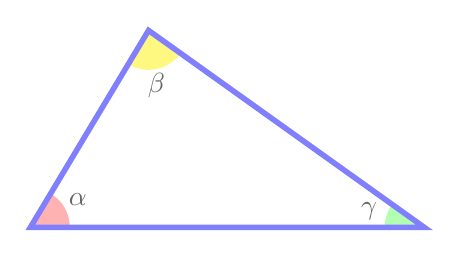
\begin{tikzpicture}
\tikzstyle{texto}=[draw=none,fill=none,black!60!white]
\tikzstyle{line}=[blue!50!white,line width=2pt]
\tikzstyle{angleA}=[draw=none,fill=red!30!white]
\tikzstyle{angleB}=[draw=none,fill=green!30!white]
\tikzstyle{angleC}=[draw=none,fill=yellow!50!white]

\draw[angleA] (0,0) -- (0:0.5) arc (0:60:0.5);

\begin{scope}[shift={(5,0)}]
    \draw[angleB] (0,0) -- (145:0.5) arc (145:180:0.5);
\end{scope}

\begin{scope}[shift={(1.5,2.5)}]
    \draw[angleC] (0,0) -- (240:0.5) arc (240:325:0.5);
\end{scope}

\draw[line] (0,0) -- (5,0) -- (1.5,2.5) -- cycle;

\node[texto] at (0.6,0.35) {\textbf{$\alpha$}};
\node[texto] at (4.3,0.2) {\textbf{$\gamma$}};
\node[texto] at (1.6,1.8) {\textbf{$\beta$}};
\end{tikzpicture}
\end{center}

$$\alpha + \beta + \gamma = \ang{180}$$

Conhecendo dois ângulos, o terceiro é sempre determinado:

$$\boxed{x = \ang{180} - \alpha - \beta}$$

A propriedade tem diversas aplicações: resolução de problemas geométricos, construção civil, navegação e desenvolvimento de identidades trigonométricas.

%%% ─── DEMONSTRAÇÃO ─────────────────────────────────────────────
\TM{Por que a soma é \ang{180}?}

Trace pelo vértice $C$ uma reta $r$ paralela à base $AB$. Por propriedades de retas paralelas cortadas por transversais, os ângulos alternos internos são iguais. Assim, $\alpha$, $\beta$ e $\gamma$ formam juntos um ângulo raso ($\ang{180}$).

\begin{center}
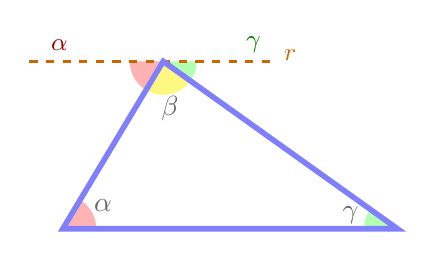
\begin{tikzpicture}[scale=0.85]
\tikzstyle{texto}=[draw=none,fill=none,black!60!white]
\tikzstyle{line}=[blue!50!white,line width=2pt]
\tikzstyle{paralela}=[orange!80!black,line width=1.2pt,dashed]
\tikzstyle{angleA}=[draw=none,fill=red!30!white]
\tikzstyle{angleG}=[draw=none,fill=green!30!white]
\tikzstyle{angleB}=[draw=none,fill=yellow!50!white]

% Ângulo α em A (vermelho)
\draw[angleA] (0,0) -- (0:0.5) arc (0:60:0.5);

% Ângulo γ em B (verde)
\begin{scope}[shift={(5,0)}]
    \draw[angleG] (0,0) -- (145:0.5) arc (145:180:0.5);
\end{scope}

% Em C: ângulo alternos α (esquerda) e γ (direita) + β (meio)
\begin{scope}[shift={(1.5,2.5)}]
    \draw[angleA] (0,0) -- (180:0.5) arc (180:239:0.5); % ≡ α
    \draw[angleB] (0,0) -- (240:0.5) arc (240:325:0.5); % β
    \draw[angleG] (0,0) -- (325:0.5) arc (325:360:0.5); % ≡ γ
\end{scope}

% Reta paralela r através de C
\draw[paralela] (-0.5,2.5) -- (3.2,2.5);
\node[orange!80!black] at (3.4,2.6) {\small $r$};

% Triângulo
\draw[line] (0,0) -- (5,0) -- (1.5,2.5) -- cycle;

% Rótulos
\node[texto] at (0.6,0.35) {\textbf{$\alpha$}};
\node[texto] at (4.3,0.2)  {\textbf{$\gamma$}};
\node[texto] at (1.6,1.8)  {\textbf{$\beta$}};
\node[red!60!black]   at (-0.05,2.75) {\small $\alpha$};
\node[green!50!black] at (2.85,2.75)  {\small $\gamma$};
\end{tikzpicture}
\end{center}

%%% ─── EXEMPLO 1 ────────────────────────────────────────────────
\TM{Exemplo:}

\begin{center}
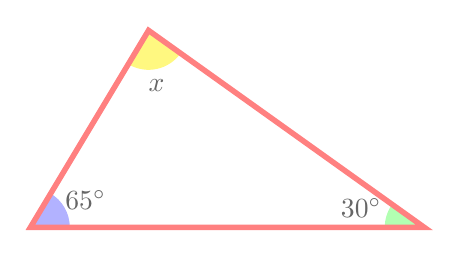
\begin{tikzpicture}
\tikzstyle{texto}=[draw=none,fill=none,black!60!white]
\tikzstyle{line}=[red!50!white,line width=2pt]
\tikzstyle{angleA}=[draw=none,fill=blue!30!white]
\tikzstyle{angleB}=[draw=none,fill=green!30!white]
\tikzstyle{angleC}=[draw=none,fill=yellow!50!white]

\draw[angleA] (0,0) -- (0:0.5) arc (0:60:0.5);

\begin{scope}[shift={(5,0)}]
    \draw[angleB] (0,0) -- (145:0.5) arc (145:180:0.5);
\end{scope}

\begin{scope}[shift={(1.5,2.5)}]
    \draw[angleC] (0,0) -- (240:0.5) arc (240:325:0.5);
\end{scope}

\draw[line] (0,0) -- (5,0) -- (1.5,2.5) -- cycle;

\node[texto] at (0.7,0.35) {\textbf{$\ang{65}$}};
\node[texto] at (4.2,0.25) {\textbf{$\ang{30}$}};
\node[texto] at (1.6,1.8) {\textbf{$x$}};
\end{tikzpicture}
\end{center}

$65 + 30 + x = 180$

$95 + x = 180$

$x= 180 - 95$

$x = \ang{85}$

%%% ─── TRIÂNGULO ISÓSCELES ──────────────────────────────────────
\TM{Triângulo Isósceles:}

O triângulo isósceles possui dois lados com a mesma medida. O terceiro lado que possui medida diferente é chamado de base. Os dois ângulos formados pela base e os lados congruentes possuem a mesma medida.

\begin{center}
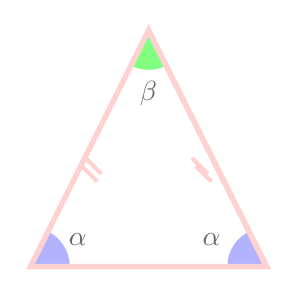
\begin{tikzpicture}
\tikzstyle{texto}=[draw=none,fill=none,black!60!white]
\tikzstyle{line}=[pink!70!white,line width=2pt]
\tikzstyle{angleA}=[draw=none,fill=blue!30!white]
\tikzstyle{angleC}=[draw=none,fill=green!50!white]

\draw[angleA] (0,0) -- (0:0.5) arc (0:65:0.5);

\begin{scope}[shift={(3,0)}]
    \draw[angleA] (0,0) -- (115:0.5) arc (115:180:0.5);
\end{scope}

\begin{scope}[shift={(1.5,3)}]
    \draw[angleC] (0,0) -- (245:0.5) arc (245:295:0.5);
\end{scope}

\draw[line] (0,0) -- (3,0) -- (1.5,3) -- cycle;

% Marcas de lado igual
\draw[pink!70!white,line width=1.5pt] (0.65,1.28) -- (0.85,1.08);
\draw[pink!70!white,line width=1.5pt] (0.70,1.38) -- (0.90,1.18);
\draw[pink!70!white,line width=1.5pt] (2.10,1.28) -- (2.30,1.08);
\draw[pink!70!white,line width=1.5pt] (2.05,1.38) -- (2.25,1.18);

\node[texto] at (0.6,0.35) {\textbf{$\alpha$}};
\node[texto] at (2.3,0.35) {\textbf{$\alpha$}};
\node[texto] at (1.5,2.2) {\textbf{$\beta$}};
\end{tikzpicture}
\end{center}

%%% ─── EXEMPLO ISÓSCELES ────────────────────────────────────────
\TM{Exemplo:}

\begin{center}
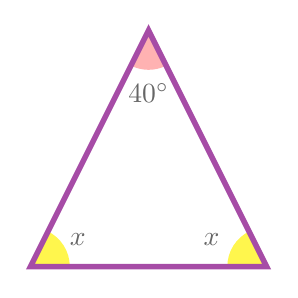
\begin{tikzpicture}
\tikzstyle{texto}=[draw=none,fill=none,black!60!white]
\tikzstyle{line}=[violet!70!white,line width=2pt]
\tikzstyle{angleA}=[draw=none,fill=yellow!70!white]
\tikzstyle{angleB}=[draw=none,fill=red!30!white]

\draw[angleA] (0,0) -- (0:0.5) arc (0:65:0.5);

\begin{scope}[shift={(3,0)}]
    \draw[angleA] (0,0) -- (115:0.5) arc (115:180:0.5);
\end{scope}

\begin{scope}[shift={(1.5,3)}]
    \draw[angleB] (0,0) -- (245:0.5) arc (245:295:0.5);
\end{scope}

\draw[line] (0,0) -- (3,0) -- (1.5,3) -- cycle;

\node[texto] at (0.6,0.35) {\textbf{$x$}};
\node[texto] at (2.3,0.35) {\textbf{$x$}};
\node[texto] at (1.5,2.2) {\textbf{$\ang{40}$}};
\end{tikzpicture}
\end{center}

$x + x + 40 = 180$

$2 x + 40 = 180$

$2 x  = 180 - 40$

$2x  = 140$

\vspace{8px}
$x  = \dfrac{140}{2}$ \vspace{8px}

$x  = \ang{70}$

%%% ─── TRIÂNGULO EQUILÁTERO ─────────────────────────────────────
\TM{Triângulo Equilátero:}

O triângulo equilátero possui os três lados com a mesma medida. Como caso especial do isósceles, seus três ângulos internos são iguais. Usando a propriedade da soma:

$$\alpha = \beta = \gamma = \dfrac{\ang{180}}{3} = \ang{60}$$

\begin{center}
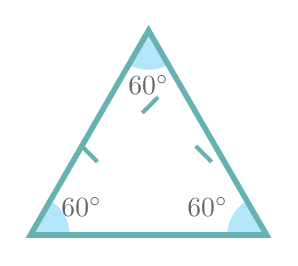
\begin{tikzpicture}
\tikzstyle{texto}=[draw=none,fill=none,black!60!white]
\tikzstyle{line}=[teal!60!white,line width=2pt]
\tikzstyle{angle60}=[draw=none,fill=cyan!30!white]

% Triângulo equilátero: A=(0,0), B=(3,0), C=(1.5, 2.598)
\draw[angle60] (0,0) -- (0:0.5) arc (0:60:0.5);

\begin{scope}[shift={(3,0)}]
    \draw[angle60] (0,0) -- (120:0.5) arc (120:180:0.5);
\end{scope}

\begin{scope}[shift={(1.5,2.598)}]
    \draw[angle60] (0,0) -- (240:0.5) arc (240:300:0.5);
\end{scope}

\draw[line] (0,0) -- (3,0) -- (1.5,2.598) -- cycle;

% Marcas de lado igual (três lados)
\draw[teal!60!white,line width=1.5pt] (0.65,1.13) -- (0.85,0.93);
\draw[teal!60!white,line width=1.5pt] (1.42,1.55) -- (1.62,1.75);
\draw[teal!60!white,line width=1.5pt] (2.10,1.13) -- (2.30,0.93);

\node[texto] at (0.65,0.35) {\textbf{$\ang{60}$}};
\node[texto] at (2.25,0.35) {\textbf{$\ang{60}$}};
\node[texto] at (1.5,1.9)   {\textbf{$\ang{60}$}};
\end{tikzpicture}
\end{center}

%%% ─── CLASSIFICAÇÃO POR ÂNGULOS ────────────────────────────────
\TM{Classificação por ângulos:}

Todo triângulo pertence a uma das três categorias abaixo de acordo com seus ângulos internos:

\begin{itemize}
    \item \textbf{Acutângulo}: todos os três ângulos são \textbf{menores} que $\ang{90}$.
    \item \textbf{Retângulo}: possui exatamente um ângulo de $\ang{90}$ (ângulo reto). Os outros dois somam $\ang{90}$ e são chamados de \textbf{ângulos complementares}.
    \item \textbf{Obtusângulo}: possui exatamente um ângulo \textbf{maior} que $\ang{90}$. Os outros dois são necessariamente agudos.
\end{itemize}

\begin{center}
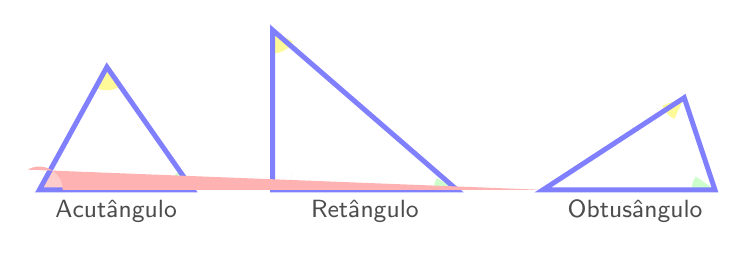
\begin{tikzpicture}[scale=0.78]
\tikzstyle{lbl}=[font=\small,black!70]
\tikzstyle{ang}=[draw=none]

%--- Acutângulo (60°, 70°, 50°): A=(0,0) B=(2.5,0) C=(1.1,2)
\draw[ang,fill=red!20!white] (0,0) -- (0:0.38) arc(0:61:0.38) -- cycle;
\begin{scope}[shift={(2.5,0)}]
\draw[ang,fill=green!20!white] (0,0) -- (125:0.38) arc(125:180:0.38) -- cycle;
\end{scope}
\begin{scope}[shift={(1.1,2)}]
\draw[ang,fill=yellow!40!white] (0,0) -- (241:0.38) arc(241:310:0.38) -- cycle;
\end{scope}
\draw[blue!50!white,line width=1.8pt] (0,0) -- (2.5,0) -- (1.1,2) -- cycle;
\node[lbl] at (1.25,-0.35) {Acutângulo};

%--- Retângulo (90°, 60°, 30°): A=(3.8,0) B=(6.8,0) C=(3.8,2.6)
\draw[ang,fill=blue!20!white] (3.8,0) -- ++(0:0.3) -- ++(90:0.3) -- ++(-90:0.3) -- cycle; % right angle mark
\begin{scope}[shift={(6.8,0)}]
\draw[ang,fill=green!20!white] (0,0) -- (150:0.38) arc(150:180:0.38) -- cycle;
\end{scope}
\begin{scope}[shift={(3.8,2.6)}]
\draw[ang,fill=yellow!40!white] (0,0) -- (270:0.38) arc(270:330:0.38) -- cycle;
\end{scope}
\draw[blue!50!white,line width=1.8pt] (3.8,0) -- (6.8,0) -- (3.8,2.6) -- cycle;
\node[lbl] at (5.3,-0.35) {Retângulo};

%--- Obtusângulo (120°, 35°, 25°): A=(8.2,0) B=(11,0) C=(10.5,1.5)
\draw[ang,fill=red!30!white] (8.2,0) -- (0:0.38) arc(0:120:0.38) -- cycle;
\begin{scope}[shift={(11,0)}]
\draw[ang,fill=green!20!white] (0,0) -- (145:0.38) arc(145:180:0.38) -- cycle;
\end{scope}
\begin{scope}[shift={(10.5,1.5)}]
\draw[ang,fill=yellow!40!white] (0,0) -- (200:0.38) arc(200:245:0.38) -- cycle;
\end{scope}
\draw[blue!50!white,line width=1.8pt] (8.2,0) -- (11,0) -- (10.5,1.5) -- cycle;
\node[lbl] at (9.7,-0.35) {Obtusângulo};

\end{tikzpicture}
\end{center}

%%% ─── ÂNGULO EXTERNO ────────────────────────────────────────────
\TM{Ângulo Externo}

Em todo triângulo, qualquer ângulo externo é igual à soma dos ângulos internos não adjacentes.

\begin{center}
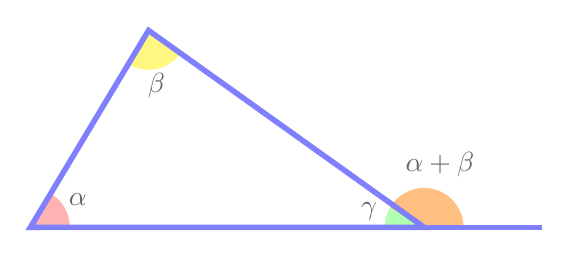
\begin{tikzpicture}
\tikzstyle{texto}=[draw=none,fill=none,black!60!white]
\tikzstyle{line}=[blue!50!white,line width=2pt]
\tikzstyle{angleA}=[draw=none,fill=red!30!white]
\tikzstyle{angleB}=[draw=none,fill=green!30!white]
\tikzstyle{angleC}=[draw=none,fill=yellow!50!white]
\tikzstyle{angleD}=[draw=none,fill=orange!50!white]

\draw[angleA] (0,0) -- (0:0.5) arc (0:60:0.5);

\begin{scope}[shift={(5,0)}]
    \draw[angleB] (0,0) -- (145:0.5) arc (145:180:0.5);
\end{scope}

\begin{scope}[shift={(1.5,2.5)}]
    \draw[angleC] (0,0) -- (240:0.5) arc (240:325:0.5);
\end{scope}

\begin{scope}[shift={(5,0)}]
    \draw[angleD] (0,0) -- (0:0.5) arc (0:150:0.5);
\end{scope}

\draw[line] (0,0) -- (5,0) -- (1.5,2.5) -- cycle;
\draw[line] (5,0) -- (6.5,0);

\node[texto] at (0.6,0.35) {\textbf{$\alpha$}};
\node[texto] at (4.3,0.2) {\textbf{$\gamma$}};
\node[texto] at (1.6,1.8) {\textbf{$\beta$}};
\node[texto] at (5.2,0.8) {\textbf{$\alpha + \beta$}};
\end{tikzpicture}
\end{center}

%%% ─── EXEMPLO ÂNGULO EXTERNO ───────────────────────────────────
\TM{Exemplo:}

Dois ângulos internos de um triângulo medem $\ang{50}$ e $\ang{70}$. Qual é o ângulo externo no terceiro vértice?

\begin{center}
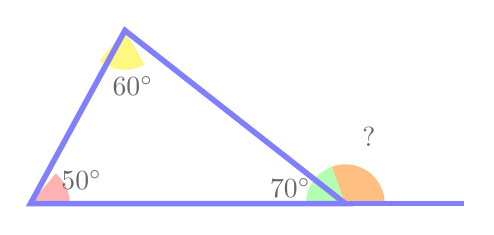
\begin{tikzpicture}
\tikzstyle{texto}=[draw=none,fill=none,black!60!white]
\tikzstyle{line}=[blue!50!white,line width=2pt]
\tikzstyle{angleA}=[draw=none,fill=red!30!white]
\tikzstyle{angleB}=[draw=none,fill=green!30!white]
\tikzstyle{angleC}=[draw=none,fill=yellow!50!white]
\tikzstyle{angleD}=[draw=none,fill=orange!50!white]

% Triângulo com ângulos 50°, 60°, 70°
% A=(0,0) ângulo≈50°, B=(4,0) ângulo≈70°, C=(1.2,2.2) ângulo≈60°
\draw[angleA] (0,0) -- (0:0.5) arc (0:50:0.5);

\begin{scope}[shift={(4,0)}]
    \draw[angleB] (0,0) -- (110:0.5) arc (110:180:0.5);
\end{scope}

\begin{scope}[shift={(1.2,2.2)}]
    \draw[angleC] (0,0) -- (230:0.5) arc (230:300:0.5);
\end{scope}

% Ângulo externo em B
\begin{scope}[shift={(4,0)}]
    \draw[angleD] (0,0) -- (0:0.5) arc (0:110:0.5);
\end{scope}

\draw[line] (0,0) -- (4,0) -- (1.2,2.2) -- cycle;
\draw[line] (4,0) -- (5.5,0);

\node[texto] at (0.65,0.3) {\textbf{$\ang{50}$}};
\node[texto] at (3.3,0.2)  {\textbf{$\ang{70}$}};
\node[texto] at (1.3,1.5)  {\textbf{$\ang{60}$}};
\node[texto] at (4.3,0.85) {\textbf{$?$}};
\end{tikzpicture}
\end{center}

\text{ângulo externo} $= \ang{50} + \ang{70} = \ang{120}$

\end{multicols}

\lfoot{\scriptsize © Copyright, Pratique Já}
\cfoot{\large \textcolor{bluebell}{pratiqueja.com}}
\end{document}
